\documentclass{article}

% Paquetes plantilla
\usepackage[square, numbers, sort]{natbib}
% \usepackage{cite}
\usepackage{graphicx}
\usepackage[utf8]{inputenc}
\usepackage{amsmath,amssymb,amsfonts}
\usepackage{algorithmic}
\usepackage{textcomp}
\usepackage{subfig}
\usepackage{float}
\usepackage{graphicx}   % Para incluir gráficos
\usepackage{subcaption} % Paquete necesario para subfiguras

\usepackage{empheq}
\usepackage{mathtools}
\usepackage[spanish]{babel}
\usepackage[paper=a4paper,margin=2.75cm]{geometry}
\usepackage{booktabs} % for tables
\usepackage[colorlinks = true,
            linkcolor = blue,
            urlcolor  = blue,
            citecolor = orange,
            anchorcolor = blue]{hyperref} % for hyperlinks
\usepackage{xcolor} % text colors
% Paquetes extra
\usepackage{subcaption, booktabs, siunitx, tikz}
\usepackage{pgfplots}
\pgfplotsset{compat=1.15}
\usepackage{mathrsfs}
\usetikzlibrary{arrows}
\tikzset{every picture/.style={line width=0.75pt}} %set default line width to 0.75pt 

\sisetup{
    round-mode          = places, % Rounds numbers
    round-precision     = 2, % to 2 places
}

\usepackage{titlesec}

\setcounter{secnumdepth}{4}

\titleformat{\paragraph}
{\normalfont\normalsize\bfseries}{\theparagraph}{1em}{}
\titlespacing*{\paragraph}
{0pt}{3.25ex plus 1ex minus .2ex}{1.5ex plus .2ex}

% Directorio con imagenes
\graphicspath{{./figs/}}

% Cabecera del documento
% ======================================================================

% Titulo
\title{PROYECTO INTEGRADOR DE AUTÓMATAS Y CONTROL DISCRETO}

% Autores
\author{Juan Pablo Sibecas \\ juan.sibecas@gmail.com \\Matias Gaviño\\ matias.linares.g@gmail.com \\ Autómatas y Control Discreto, Facultad de Ingeniería, \\ Universidad Nacional de Cuyo, \\ Mendoza, Argentina}

% Fecha
\date{Junio de 2024}

% Cuerpo del documento
% ======================================================================
\begin{document}

% Comandos definidos por el autor
\renewcommand{\tablename}{Tabla}
% \renewcommand{\color{blue}{#1}}{\azul}

% Crear cabecera
\maketitle

% Resumen
% ======================================================================
\begin{abstract}\label{sec:abstract}

En este informe se presenta el desarrollo e implementación de un sistema de control y protección para una grúa portuaria de tipo pórtico, como parte del Proyecto Global Integrador 317 AyCD. El proyecto integra un enfoque híbrido de control distribuido, empleando Matlab/Simulink y Codesys para diseñar, simular y validar el sistema. El control consta de tres niveles: control continuo para el manejo de las principales dinámicas de traslación e izaje, un nivel supervisor encargado de la secuencia lógica de estados, y un nivel de seguridad para la protección de los componentes y del entorno operativo.

Los resultados obtenidos a partir de simulaciones y pruebas en un entorno de PLC demostraron la efectividad del control manual y automático para seguir trayectorias específicas, manteniendo la estabilidad de la carga y minimizando las oscilaciones. Además, el sistema de protección logró actuar eficazmente en situaciones de emergencia, garantizando la seguridad durante las operaciones.

Este proyecto no solo ha alcanzado los objetivos planteados, sino que también ha demostrado la viabilidad de una solución de control que optimiza el rendimiento y seguridad de una grúa portuaria.



\end{abstract}

\newpage

% Insertar la tabla de contenidos
\tableofcontents

% Iniciar las secciones del documento
\newpage

\section{Introducción} \label{sec:intro}


El presente informe aborda el control de una grúa portuaria destinada a la carga, descarga y reubicación de contenedores entre el barco y las bahías de carga. El objetivo es mejorar la eficiencia del sistema mediante trayectorias de movimiento que sean tanto suaves como rápidas.

Para desarrollar este control, se comienza con el modelado del sistema físico, que consta de un carro para el movimiento horizontal y un sistema de izaje para el movimiento vertical. Ambos movimientos están acoplados por la carga, la cual consiste en un contenedor y un "spreader" que lo sostiene. La traslación y el izaje son accionados por motores eléctricos, lo que permite un control preciso de las trayectorias.

El desarrollo del informe incluye el modelado del sistema físico, obteniendo las ecuaciones de movimiento y utilizando Simulink para simular su comportamiento. A continuación, se diseña un control híbrido de tres niveles: el nivel 2 se encarga del control en tiempo discretizado para los motores que accionan el izaje y el carro; el nivel 1 consiste en un controlador discreto basado en eventos, que genera trayectorias suaves y eficientes; y el nivel 0 actúa como sistema de seguridad, asegurando que el sistema entre en un estado seguro en caso de fallas. Para la simulación del controlador, se emplea el software Matlab/Simulink, y luego se implementa en Codesys para simular su ejecución en un PLC.


\section{Desarrollo} \label{sec:desarrollo}
    \subsection{Modelo del Sistema Físico} \label{sec:plantModel}

        El modelo del sistema se simplifica para controlar la posición de la carga en un plano. No se considerarán los grados de libertad fuera del plano perpendicular al eje longitudinal del muelle. Se asume que la estructura de la grúa es rígida y no presenta vibraciones, a diferencia de los cables, que se consideran flexibles.

        El desarrollo de las ecuaciones se basa en lo presentado en el enunciado del trabajo práctico.
    
        
        \subsubsection{Subsistema de Izaje}
            La dinámica del subsistema de izaje se modela utilizando la segunda ley de Newton para el tambor y el motor:

            \textbf{Segunda ley de Newton para el tambor:}
            \begin{equation} \label{eq:tamborIzaje}
                J_{hd+hEb} \frac{d \omega_{hd}}{dt} = T_{hd}(t) + T_{hEb}(t) - b_{hd} \omega_{hd}(t) - T_{hdl}(t)
            \end{equation}

            \textbf{Segunda ley de Newton para el motor:}
            \begin{equation} \label{eq:motorIzaje}
                J_{hm+hb} \frac{d \omega_{hm}}{dt} = T_{hm}(t) + T_{hb}(t) - b_{hm} \omega_{hm}(t) - T_{hml}(t)
            \end{equation}

            \textbf{Relación de transmisión:}
            \begin{equation} \label{eq:transmisionIzaje}
                i_h = \frac{\omega_{hm}(t)}{\omega_{hd}(t)} = \frac{T_{hd}(t)}{T_{hml}(t)}
            \end{equation}

            Sustituyendo la ecuación \ref{eq:transmisionIzaje} en \ref{eq:motorIzaje} y despejando $T_{hd}(t)$, se obtiene:

            \begin{equation} \label{eq:Thd}
                T_{hd}(t) = J_{hm+hb} \frac{d \omega_{hd}}{dt} {i_h}^2 - b_{hm} \omega_{hd}(t) {i_h}^2 + i_h (T_{hm}(t) + T_{hb}(t))
            \end{equation}

            Reemplazando en \ref{eq:tamborIzaje} y operando se obtiene:

            \begin{equation} \label{eq:izajeThdl}
                (J_{hd+hEb} + J_{hm+hb} i_h^2) \frac{d \omega_{hd}}{dt} = - (b_{hd} + b_{hm} i_h^2) \omega_{hd}(t) + i_h (T_{hm}(t) + T_{hb}(t)) + T_{hEb}(t) - T_{hdl}(t)
            \end{equation}

            Considerando que $T_{hdl}(t) = F_{hw}(t) \cdot r_{hd}$, $2V_h = r_{hd} \cdot \omega_{hd}(t)$ y $V_h = -\frac{d l_h(t)}{dt}$, dividiendo por $r_{hd}$:

            \begin{equation} \label{eq:izajeFhw}
                2\frac{(J_{hd+hEb} + J_{hm+hb} i_h^2)}{r_{hd}^2} \frac{d^2 l_h(t)}{dt^2} = - 2\frac{(b_{hd} + b_{hm} i_h^2)}{r_{hd}^2} \frac{d l_h(t)}{dt} - \frac{i_h}{r_{hd}} (T_{hm}(t) + T_{hb}(t)) - \frac{T_{hEb}(t)}{r_{hd}} + F_{hw}(t)
            \end{equation}

            Reemplazando por parámetros equivalentes:

            \begin{equation} \label{eq:izajeEquiv}
                M_{Eh} \ddot{l_h}(t) = - b_{Eh} \dot{l_h}(t) - \frac{i_h}{r_{hd}} (T_{hm}(t) + T_{hb}(t)) - \frac{T_{hEb}(t)}{r_{hd}} + F_{hw}(t)
            \end{equation}

            Donde:

            \begin{align} \label{eq:izajeParamsEquiv}
                M_{Eh} &= 2\frac{(J_{hd+hEb} + J_{hm+hb} i_h^2)}{r_{hd}^2} \\
                b_{Eh} &= 2\frac{(b_{hd} + b_{hm} i_h^2)}{r_{hd}^2}
            \end{align}

            En la Figura \ref{fig:hoisting_drive_simulink} se presenta el modelo de Simulink del subsistema de izaje. En este modelo se implementa la ecuación \ref{eq:izajeEquiv} junto con los correspondientes parámetros equivalentes. Además, se incluye el modelo del sistema de freno y del freno de emergencia.

            \begin{figure} [H]
                \centering
                \includegraphics[width=1\textwidth]{figs/hoisting_drive_simulink.png}
                \caption{Modelo de Simulink del subsistema de izaje}
                \label{fig:hoisting_drive_simulink}
            \end{figure}

            \textbf{Modelo del cable de izaje}

            El modelo del cable de izaje se obtiene a partir de la ecuación 2/2.a. Se considera que el cable solo soporta cargas de tracción, por lo que si el resultado de la tensión obtenido de dicha ecuación es negativo, se toma como cero. En la Figura \ref{fig:hoisting_cable_mode_simulink} se presenta el modelo implementado en Simulink del cable de izaje.

            \begin{figure} [H]
                \centering
                \includegraphics[width=1\textwidth]{figs/hoisting_cable_mode_simulink.png}
                \caption{Modelo de Simulink del cable de izaje}
                \label{fig:hoisting_cable_mode_simulink}
            \end{figure}



            \subsubsection{Subsistema Carro}

            El subsistema del carro se modela considerando tres subcomponentes principales: el motor, el tambor y el cable. En la Figura \ref{fig:trolley_drive_simulink} se muestra el modelo de Simulink que representa estos subsistemas.
            
            \begin{figure} [H]
                \centering
                \includegraphics[width=1\textwidth]{figs/trolley_drive_simulink.png}
                \caption{Modelo de Simulink del subsistema del carro}
                \label{fig:trolley_drive_simulink}
            \end{figure}
            
            \textbf{Motor del carro}
            
            El modelo del motor se obtiene a partir de la ecuación 4 del enunciado. En la Figura \ref{fig:trolley_subsystem_simulink} se presenta el modelo implementado en Simulink.
            
            \begin{figure} [H]
                \centering
                \includegraphics[width=1\textwidth]{figs/trolley_subsystem_simulink.png}
                \caption{Modelo de Simulink del motor del subsistema carro}
                \label{fig:trolley_subsystem_simulink}
            \end{figure}
            
            \textbf{Tambor del carro}
            
            La dinámica del tambor del carro se describe usando la segunda ley de Newton:
            
            \textbf{Ecuación para el tambor:}
            \begin{equation} \label{eq:tamborCarro}
                J_{td} \frac{d \omega_{td}(t)}{dt} = T_{td}(t) - b_{td} \omega_{td}(t) - T_{tdl}(t)
            \end{equation}
            
            \textbf{Ecuación para el motor:}
            \begin{equation} \label{eq:motorCarro}
                J_{tm+tb} \frac{d \omega_{tm}(t)}{dt} = T_{tm}(t) + T_{tb}(t) - b_{tm} \omega_{tm}(t) - T_{tml}(t)
            \end{equation}
            
            \textbf{Relación de transmisión:}
            \begin{equation} \label{eq:transmisionCarro}
                i_t = \frac{\omega_{tm}(t)}{\omega_{td}(t)} = \frac{T_{td}(t)}{T_{tml}(t)}
            \end{equation}
            
            Reemplazando la ecuación \ref{eq:transmisionCarro} en \ref{eq:motorCarro} y despejando $T_{td}(t)$, se tiene:
            
            \begin{equation} \label{eq:Ttd}
                T_{td}(t) = J_{tm+tb} \frac{d \omega_{td}(t)}{dt} {i_t}^2 - b_{tm} \omega_{td}(t) {i_t}^2 + i_t (T_{tm}(t) + T_{tb}(t))
            \end{equation}
            
            Sustituyendo \ref{eq:Ttd} en \ref{eq:tamborCarro} y reorganizando:
            
            \begin{equation} \label{eq:carroTtdl}
                (J_{td} + J_{tm+tb} i_t^2) \frac{d \omega_{td}(t)}{dt} = i_t (T_{tm}(t) + T_{tb}(t)) - (b_{td} + b_{tm} i_t^2) \omega_{td}(t) - T_{tdl}(t)
            \end{equation}
            
            Considerando que $\omega_{td}(t) \cdot r_{td} = V_{td}(t)$, $F_{tw}(t) \cdot r_{td} = T_{tdl}(t)$ y $V_{td}(t) = \frac{d x_{td}}{dt}$, dividiendo por $r_{td}$:
            
            \begin{equation} \label{eq:carroFtw}
                \frac{(J_{td} + J_{tm+tb} i_t^2)}{r_{td}^2} \frac{d^2 x_{td}(t)}{dt^2} = - \frac{(b_{td} + b_{tm} i_t^2)}{r_{td}^2} \frac{d x_{td}(t)}{dt} + \frac{i_t}{r_{td}} (T_{tm}(t) + T_{tb}(t)) - F_{tw}(t)
            \end{equation}
            
            Reemplazando por parámetros equivalentes, se obtiene la ecuación del tambor del subsistema carro:
            
            \begin{equation} \label{eq:TamborCarro}
                M_{Etd} \ddot{x_{td}}(t) = - b_{Etd} \dot{x_{td}}(t) + \frac{i_t}{r_{td}} (T_{tm}(t) + T_{tb}(t)) - F_{tw}(t)
            \end{equation}
            
            \textbf{Ecuación de movimiento del carro:}
            
            \begin{equation} \label{eq:Carro}
                M_t \ddot{x_{t}}(t) = - b_t \dot{x_{t}}(t) + F_{tw}(t) + 2 F_{hw}(t) \sin{\theta_l(t)}
            \end{equation}
            
            \textbf{Fuerza transmitida por el cable del carro:}
            
            \begin{equation} \label{eq:fuerzaCableCarro}
                F_{tw}(t) = K_{tw}(x_{td}(t) - x_t(t)) + b_{tw}(\dot{x_{td}}(t) - \dot{x_t}(t))
            \end{equation}
            
            En la Figura \ref{fig:trolley_drum_mode_simulink} se muestra el modelo de Simulink que corresponde a la ecuación \ref{eq:Carro} con los parámetros equivalentes correspondientes. Además, se incluye el modelo del freno del tambor.
            
            \begin{figure} [H]
                \centering
                \includegraphics[width=1\textwidth]{figs/trolley_drum_subsystem_simulink.png}
                \caption{Modelo de Simulink del tambor del subsistema carro}
                \label{fig:trolley_drum_mode_simulink}
            \end{figure}
            
            \textbf{Modelo del cable del carro}
            
            La Figura \ref{fig:trolley_cable_mode_simulink} muestra el modelo de Simulink del cable del subsistema carro, en el que se implementa la ecuación 4.a del enunciado.
            
            \begin{figure} [H]
                \centering
                \includegraphics[width=1\textwidth]{figs/trolley_cable_mode_simulink.png}
                \caption{Modelo de Simulink del cable del subsistema carro}
                \label{fig:trolley_cable_mode_simulink}
            \end{figure}
            



            %\textbf{Modelo los interruptores de fin de carrera}
            


            \subsubsection{Perfil de obstáculos}
            El perfil de obstaculos se modela como uma matriz de Nx2 donde la primera columna representa la posicion en x y la segunda la altura del obstáculos perfil del obstáculo. El perfil esta discgretizado en x segun un dx determinado. 
            AL iniciar la simulacion se inizializa esta matriz con el perfil de los obstáculos inmoviles. Luego se actualiza la matiz teneniendo en cuenta la cantidad de containes en cada comunma del barco o en la bahía de carga inicialmente.
            Cuando durante la simulación se recoje o se deja un contenedor se actualiza la matriz de obstáculos mediante el modelo en stateflow que se muestra en la figura \ref{fig:container_profile_stateflow}.
            \begin{figure} [H]
                \centering
                \includegraphics[width=1\textwidth]{figs/container_profile_stateflow.png}
                \caption{Modelo en stateflow de la actualización del perfil de obstáculos}
                \label{fig:container_profile_stateflow}
            \end{figure}
    
            \subsubsection{Modelo de la carga}
                
                La carga se modela teniando en cuenta la tensión del cable de izaje, así como muestran las ecuaciones 1.a y 1.b del enunciado. En la figura \ref{fig:load_simulink} se muestra el modelo de Simulink de la carga.
    
                \begin{figure} [H]
                    \centering
                    \includegraphics[width=1\textwidth]{figs/load_simulink.png}
                    \caption{Modelo de Simulink de la carga}
                    \label{fig:load_simulink}
                \end{figure}
    
                El ángulo del cable de izaje respecto de la vertical se obtiene a partir de la posicion de la carga y el carro, así como indica la ecuación 0.d del enunciado. En la figura \ref{fig:load_sway_simulink} se muestra el modelo de Simulink del balanceo de la carga.
    
                \begin{figure} [H]
                    \centering
                    \includegraphics[width=0.5\textwidth]{figs/load_sway_simulink.png}
                    \caption{Modelo de Simulink del balanceo de la carga}
                    \label{fig:load_sway_simulink}
                \end{figure}
    
                Al igual que el ángulo del cable de izaje, el largo del mismo se obtiene a partir de la posición de la carga y el carro, así como indica la ecuación 0.c del enunciado. La velocidad de cambio de esta longitud se calcula de forma analítica utilizando la ecuación 1.c'. En la figura \ref{fig:wirerope_length_simulink} se muestra el modelo de Simulink lo anteriormente mencionado.
    
                \begin{figure} [H]
                    \centering
                    \includegraphics[width=0.5\textwidth]{figs/wirerope_length_simulink.png}
                    \caption{Modelo de Simulink del largo del cable de izaje}
                    \label{fig:wirerope_length_simulink}
                \end{figure}
    
                \textbf{Modelo de la fuerza de contacto}
    
                El modelo de la fuerza de contacto se refiere al análisis de las interacciones entre la carga suspendida (spreader o contenedor) y la superficie de apoyo durante las maniobras de izaje o descenso en una grúa portuaria. Este modelo tiene en cuenta los estados del cable de izaje (tenso o flojo) y los modos de contacto (carga suspendida o apoyada). Se consideran las fuerzas de fricción horizontal y las reacciones elásticas verticales que ocurren cuando la carga toca la superficie de apoyo, así como el comportamiento dinámico del sistema para evitar tirones bruscos en el cable.
    
                El modelo se implementa en Simulink, como se muestra en la Figura \ref{fig:contact_mode_simulink}, y utiliza parámetros como la rigidez de compresión ($K_{cy}$) y la fricción ($b_{cx}, b_{cy}$) para simular las fuerzas de contacto bajo diferentes condiciones operativas. 
    
                Las ecuaciones que definen el comportamiento de la fuerza de contacto son las siguientes:
    
                \begin{equation}
                F_{cx}(t) = -b_{cx} \cdot v_{lx}(t)
                \end{equation}
    
                \begin{equation}
                F_{cy}(t) = K_{cy} \cdot (y_{c0}(x_l, t) - (y_l(t) - h_c(TLK))) - b_{cy} \cdot v_{ly}(t)
                \end{equation}
    
                Donde:
                \begin{itemize}
                    \item $F_{cx}$ es la fuerza de fricción horizontal.
                    \item $F_{cy}$ es la fuerza de reacción elástica vertical.
                    \item $b_{cx}$ y $b_{cy}$ son los coeficientes de fricción horizontal y vertical, respectivamente.
                    \item $K_{cy}$ es la rigidez de compresión vertical.
                    \item $v_{lx}$ y $v_{ly}$ son las velocidades horizontales y verticales de la carga.
                    \item $y_{c0}(x_l, t)$ representa el perfil de obstáculos o la altura de apoyo vertical.
                    \item $h_c(TLK)$ indica la altura inferior de la carga, dependiendo del estado de los twistlocks (abiertos o cerrados).
                \end{itemize}
    
                \begin{figure}
                    \centering
                    \includegraphics[width=0.5\textwidth]{figs/contact_mode_simulink.png}
                    \caption{Modelo de Simulink de la fuerza de contacto}
                    \label{fig:contact_mode_simulink}
                \end{figure}
                
        \subsection{Diseño del controlador}

            En esta sección se presenta el desarrollo de los controladores para los distintos subsistemas de la grúa portuaria. Cada controlador se diseña para asegurar un desempeño eficiente y seguro, cumpliendo con las especificaciones operativas del sistema. Los subsistemas controlados incluyen el carro, el mecanismo de izaje y el balanceo de la carga, abordados en las siguientes subsecciones.

            \subsubsection{Control del Carro} 

            Según el modelo del sistema, la ecuación de movimiento del carro se describe por:
            
            \begin{equation}
                M_t \ddot{x_{t}}(t) = - b_E \dot{x_{t}}(t) + \frac{i_t}{r_{td}} T_{tm}(t) - F_{L}(t) 
            \end{equation}
            
            Para simplificar el análisis, se desacopla el primer término sustituyendo:
            
            \begin{equation}
            T_m(t) = T_{tm}^*(t) + \frac{r_{td} b_E}{i_t} \dot{x_t}(t)
            \end{equation}
            
            Cuando se desprecia la fuerza externa $F_{L}(t)$, se obtiene la ecuación simplificada:
            
            \begin{equation}
                M_E \ddot{x_{t}}(t) =  \frac{i_t}{r_{td}} T_{tm}^*(t) 
            \end{equation}
            
            Aplicando la transformada de Laplace y definiendo la ley de control mediante un controlador PID, se tiene:
            
            \begin{equation}
                M_E s^2 X_t(s) =  \frac{i_t}{r_{td}} T_{tm}^*(s)
            \end{equation}
            
            La expresión para $T_m^*(s)$ bajo un control PID queda definida como:
            
            \begin{equation}
                T_m^*(s) = G_T(s)\left( b_{at} + \frac{k_{sat}}{s} + \frac{k_{siat}}{s^2} \right)(v_t^*(s) - v_t(s))
            \end{equation}
            
            Sustituyendo en la ecuación del movimiento y reorganizando, se obtiene:
            
            \begin{equation}
                M_E s^2 X_t(s) =  \frac{i_t}{r_{td}} G_T(s)\left( b_{at} + \frac{k_{sat}}{s} + \frac{k_{siat}}{s^2} \right)(v_t^*(s) - v_t(s))
            \end{equation}
            
            Despejando $\frac{v_t(s)}{v_t^*(s)}$, se llega a:
            
            \begin{equation}
                \frac{v_t(s)}{v_t^*(s)} = \frac{b_{at} s^2 + k_{sat}s + k_{siat}}{s^3 \frac{r_{td}}{i_t}M_E + s^2 b_{at} + s k_{sat} + k_{siat}}
            \end{equation}
            
            Al igualar el denominador con el polinomio característico deseado, se define:
            
            \begin{equation}\label{(eq:polinomio)}
                p(s) = s^3 + \omega_n \eta s^2 + \omega_n^2 \eta s + \omega_n^3
            \end{equation}
            
            Lo que lleva a las siguientes relaciones:
            
            \begin{equation}
                \begin{cases}
                    \omega_n \eta = \frac{b_{at} i_t}{r_{td}M_E} \\
                    \omega_n^2 \eta = \frac{k_{sat} i_t}{r_{td}M_E} \\
                    \omega_n^3 = \frac{k_{siat} i_t}{r_{td}M_E}
                \end{cases}
            \end{equation}
            
            Finalmente, las constantes del controlador PID se determinan como:
            
            \begin{equation}
                \begin{cases}
                    b_{at} = \frac{r_{td}M_E \omega_n \eta}{i_t} \\
                    k_{sat} = \frac{r_{td}M_E \omega_n^2 \eta}{i_t} \\
                    k_{siat} = \frac{r_{td}M_E \omega_n^3}{i_t}
                \end{cases}
            \end{equation}
            
            Los parámetros $\omega_n$ y $\eta$ se ajustan para garantizar la estabilidad del sistema, considerando también el control del balanceo de la carga. En la Figura \ref{fig:pid_trolley_simulink}, se muestra la implementación del controlador PID en Simulink, donde se ha realizado una discretización temporal aplicando la integral por el método de trapecios.
            
            \begin{figure}[H]
                \centering
                \includegraphics[width=0.8\textwidth]{figs/PID_trolley_Simulink.png}
                \caption{Controlador PID para el carro de la grúa}
                \label{fig:pid_trolley_simulink}
            \end{figure}
            


        \subsubsection{Control del Izaje}

            De forma similar al control del carro, se obtiene la ecuación dinámica para el control del izaje:
            
            \begin{equation}
                M_{Eh} \ddot{l_h}(t) = -b_{Eh} \dot{l_h}(t) - \frac{i_h}{r_{hd}} T_{hm}(t)
            \end{equation}
            
            La ley de control PID en el dominio de Laplace es:
            
            \begin{equation}
                T_{hm}(s) = G_T(s) \left( b_{ah} + \frac{k_{sah}}{s} + \frac{k_{siah}}{s^2} \right) \left( v_h^*(s) - v_h(s) \right)
            \end{equation}
            
            Aplicando la transformada de Laplace y despejando \(\frac{v_h(s)}{v_h^*(s)}\), se obtiene:
            
            \begin{equation}
                \frac{v_h(s)}{v_h^*(s)} = \frac{b_{ah} s^2 + k_{sah} s + k_{siah}}{M_{Eh} \frac{r_{hd}}{i_h} s^3 + b_{ah} s^2 + k_{sah} s + k_{siah}}
            \end{equation}
            
            Igualando el denominador con el polinomio característico deseado:
            
            \begin{equation}
                s^3 + 2 \zeta \omega_n s^2 + \omega_n^2 s + \omega_n^3 = 0
            \end{equation}
            
            Se obtienen las siguientes ecuaciones de comparación:
            
            \begin{equation}
                \begin{cases}
                    2 \zeta \omega_n = \frac{b_{ah} i_h}{r_{hd} M_{Eh}} \\
                    \omega_n^2 = \frac{k_{sah} i_h}{r_{hd} M_{Eh}} \\
                    \omega_n^3 = \frac{k_{siah} i_h}{r_{hd} M_{Eh}}
                \end{cases}
            \end{equation}
            
            Finalmente, las constantes del controlador PID son:
            
            \begin{equation}
                \begin{cases}
                    b_{ah} = \frac{2 \zeta \omega_n r_{hd} M_{Eh}}{i_h} \\
                    k_{sah} = \frac{\omega_n^2 r_{hd} M_{Eh}}{i_h} \\
                    k_{siah} = \frac{\omega_n^3 r_{hd} M_{Eh}}{i_h}
                \end{cases}
            \end{equation}

            Finalmente, se observa en la figura \ref{fig:pid_hoist_simulink} la implementación del controlador en Simulink. Al igual que en el caso del carro, se realizó una discretización de tiempo aplicando la integral por el método de trapecios.

            \begin{figure}[H]
                \centering
                \includegraphics[width=0.8\textwidth]{figs/PID_hoist_Simulink.png}
                \caption{Controlador PID para el izaje de la grúa}
                \label{fig:pid_hoist_simulink}
            \end{figure}
        


        \subsubsection{Control de balanceo}

        \textbf{Modelo simplificado de sistema físico Péndulo-Carro}

            A continuación se derivan las ecuaciones que modelan el sistema carro-pendulo. Se utilizará el metodo de Lagrange definiendo las cordenadas generalizadas 
            \(x_t\) y \(\theta\) . Donde \(x_t\) es la posición del carro y \(\theta\) es el angulo del pendulo respecto a la vertical. 
            A modo de simplificaion se toma \(l\) como un parametro y no como una funcion del tiempo.
            El sistema se modela siguiento el modelo físico de la figura 3 del enunciado.
            \begin{figure}[H]
                \centering
                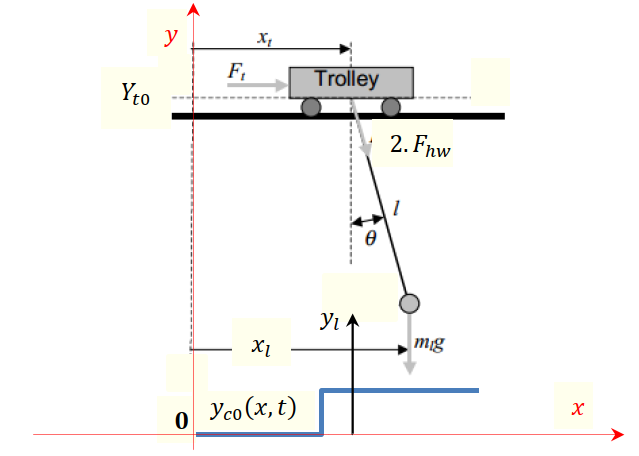
\includegraphics[width=0.5\textwidth]{figs/figure3_enunciado.png}
                \caption{Modelo físico simplificado del subsistema Carro – Cable – Carga y Perfil de Obstáculos}
                \label{fig:pendulo}
            \end{figure}
            
            \begin{equation}\label{eq:kinetic1}
                K = K_t + K_{lx} + K_{ly}
            \end{equation}
            \begin{equation}\label{eq:xl}
                x_l=x_t+l\sin{\theta}
            \end{equation}
            \begin{equation}\label{eq:dxl}
                \dot{x_l}=\dot{x_t}+l\cos{\theta}\dot{\theta}
            \end{equation}
            \begin{equation}\label{eq:y}
                y_l=Y_{t0}-l\cos{\theta}
            \end{equation}
            \begin{equation}\label{eq:dy}
                \dot{y_l}=-l\sin{\theta}\dot{\theta}
            \end{equation}

            \begin{equation}\label{eq:kinetic2}
                K = \frac{1}{2}m_t\dot{x_t}^2   +\frac{1}{2}m_l\dot{x_l}^2  +\frac{1}{2}m_l\dot{y_l}^2
            \end{equation}

            \begin{equation}\label{eq:kinetic3}
                K = \frac{1}{2}m_t\dot{x_t}^2   +\frac{1}{2}m_l(\dot{x_t}+l\cos{\theta}\dot{\theta})^2  +\frac{1}{2}m_l(-l\sin{\theta}\dot{\theta})^2
            \end{equation}

            \begin{equation}\label{eq:kinetic4}
                    K = \frac{1}{2}m_t\dot{x_t}^2 +\frac{1}{2}m_l(\dot{x_t}^2+l^2\cos^2{\theta}\dot{\theta}^2
                    +2l\dot{x_t}\cos{\theta}\dot{\theta})+\frac{1}{2}m_ll^2\sin^2{\theta}\dot{\theta}^2
            \end{equation}

            \begin{equation}\label{eq:potential}
                U = -m_lgl\cos{\theta}
            \end{equation}
            \begin{equation}\label{eq:lagrange}
                L = K - U
            \end{equation}

            \begin{equation}\label{eq:lagrange2}
                    L = \frac{1}{2}m_t\dot{x_t}^2
                    +\frac{1}{2}m_l(\dot{x_t}^2
                +l^2\cos^2{\theta}\dot{\theta}^2
                +2l\dot{x_t}\cos{\theta}\dot{\theta})
                +\frac{1}{2}m_ll^2\sin^2{\theta}\dot{\theta}^2
                +m_lgl\cos{\theta}
            \end{equation}

            \begin{equation}\label{eq:lagrange3}
                L = \frac{1}{2}m_t\dot{x_t}^2+\frac{1}{2}m_l\dot{x_t}^2
                +\frac{1}{2}m_ll^2\dot{\theta}^2
                +m_l\dot{x_t}l\cos{\theta}\dot{\theta}
                +m_lgl\cos{\theta}
            \end{equation}

            Se define el sistema de ecuaciones de Euler-Lagrange:
            \begin{equation}\label{eq:euler1}
                \frac{d}{dt}\left(\frac{\partial L}{\partial \dot{q}_i}\right)-\frac{\partial L}{\partial q_i}=Q_i
            \end{equation}

            Para \(q_i = x_t\):
            \begin{equation}\label{eq:euler2}
                \frac{d}{dt}\left(\frac{\partial L}{\partial \dot{x}_t}\right)-\frac{\partial L}{\partial x_t}=Q_t
            \end{equation}
            \begin{equation}
                \frac{\partial L}{\partial \dot{x}_t}= (m_t+m_l)\dot{x}_t+m_ll\cos{\theta}\dot{\theta}
            \end{equation}
            \begin{equation}            
                    \frac{d}{dt}\left(\frac{\partial L}{\partial \dot{x}_t}\right)= 
                    (m_t+m_l)\ddot{x}_t+m_l l\cos{\theta}\ddot{\theta}-m_ll\sin{\theta}\dot{\theta}^2
            \end{equation}
            \begin{equation}
                \frac{\partial L}{\partial x_t}=0
            \end{equation}
            Entonces:
            \begin{equation}
                (m_t+m_l)\ddot{x}_t+m_l l\cos{\theta}\ddot{\theta}-m_l l\sin{\theta}\dot{\theta}^2=F_t(t)-b_{eqt} \dot{x}_t
            \end{equation}

            Para \(q_i = \theta\):

            \begin{equation}\label{eq:euler3}
                \frac{d}{dt}\left(\frac{\partial L}{\partial \dot{\theta}}\right)-\frac{\partial L}{\partial \theta}=Q_{\theta}
            \end{equation}

            \begin{equation}
                \frac{\partial L}{\partial \dot{\theta}}=m_l\dot{x_t}l\cos{\theta}+m_ll^2\dot{\theta}
            \end{equation}

            \begin{equation}
                    \frac{d}{dt}\left(\frac{\partial L}{\partial \dot{\theta}}\right)= m_l\ddot{x_t}l\cos{\theta} -m_l\dot{x_t}l\sin{\theta}\dot{\theta}+m_ll^2\ddot{\theta}
            \end{equation}

            \begin{equation}
                \frac{\partial L}{\partial \theta}=-m_l\dot{x_t}l\sin{\theta}\dot{\theta}-m_lgl\sin{\theta}
            \end{equation}

            Entonces:
            \begin{equation}
                m_l\ddot{x_t}l\cos{\theta} -m_l\dot{x_t}l\sin{\theta}\dot{\theta}+m_ll^2\ddot{\theta}+m_l\dot{x_t}l\sin{\theta}\dot{\theta}+m_lgl\sin{\theta}=0
            \end{equation}

            Finalmente, el sistema de ecuaciones que define el modelo del sistema carro-pendulo es:
            \begin{equation}
                \begin{cases}
                    (m_t+m_l)\ddot{x}_t+m_ll\cos{\theta}\ddot{\theta}-m_ll\sin{\theta}\dot{\theta}^2=F_t(t)-b_{eqt} \dot{x}_t\\
                    m_l\ddot{x_t}l\cos{\theta} -m_l\dot{x_t}l\sin{\theta}\dot{\theta}+m_ll^2\ddot{\theta}+m_l\dot{x_t}l\sin{\theta}\dot{\theta}+m_lgl\sin{\theta}=0
                \end{cases}
            \end{equation}

            \begin{empheq}[box=\fbox]{equation}\label{eq:modeloPendulo-Carro}
                \begin{cases}
                    (m_t+m_l)\ddot{x}_t + m_l l \cos{\theta} \ddot{\theta} - m_l l \sin{\theta} \dot{\theta}^2 = F_t(t)-b_{eqt} \dot{x}_t \\
                    \ddot{x}_t \cos{\theta} + l \ddot{\theta} + g \sin{\theta} = 0
                \end{cases}
            \end{empheq}

       
        \textbf{Diseño del control de balanceo}

        Se parte de la segunda ecuación de \ref{eq:modeloPendulo-Carro} y de la ecuación que modela la dinámica del carro \ref{eq:carrosimp}.

        \begin{equation} \label{eq:carrosimp}
            M_{Etd} \ddot{x_{td}}(t) = - b_{Etd} \dot{x_{td}}(t) + F_{t}(t)
        \end{equation}

        \begin{equation}
            \frac{F_t-b_e\dot{x}_{td}}{M_{Etd}}\cos{\theta}+l \ddot{\theta}+ g \sin{\theta}=0
        \end{equation}

        Igualando con la primera ecuación de \ref{eq:modeloPendulo-Carro}

        \begin{equation} \label{eq:DC1}
            (m_t+_l)\ddot{x}_{td}+m_ll\cos{\theta}\ddot{\theta}-m_l\sin{\theta}\dot{\theta}^2=\frac{-M_{Etd}l\ddot{\theta}}{\cos{\theta}}-M_{Etd}g\tan{\theta}
        \end{equation}

        Se linealiza la ecuación \ref{eq:DC1} con respecto al punto \(\theta=\theta_0\), \(\dot{\theta}=0\), \(\ddot{\theta}=0\) y \(\ddot{x}_{td}=0\).

        \begin{equation} \label{eq:DC2}
            -m_ll\sin{\theta_0}(\theta-\theta_0)+m_ll\cos{\theta_0}\ddot{\theta}+(m_t+m_l)\ddot{x}_t=\frac{-M_{Etd}g}{\cos^2{\theta_0}}(\theta-\theta_0)-\frac{-M_{Etd}l}{\cos{\theta_0}}\ddot{\theta}
        \end{equation}

        Se realizá la transformada de Laplace y se reordenan los términos según \(\Theta(s)\) y \(V_t(s)\).

        \begin{equation} \label{eq:DC3}
            \Theta\bigg[s^2\bigg( m_ll\cos{\theta_0}+\frac{M_{Etd}l}{\cos{\theta_0}}\bigg) + \bigg( -m_l-\sin{\theta_0}+\frac{M_{Etd}g}{\cos^2{\theta_0}} \bigg) \bigg]= V_t \bigg[(m_t+m_l)s\bigg]+\frac{M_{Etd}g}{\cos^2{\theta_0}}-m_ll\sin{\theta_0}\theta_0
        \end{equation}

        Se obtiene la función de transferencia \ref{eq:DC4}:
        \begin{equation} \label{eq:DC4}
            G_c(s)=\frac{\Theta}{V_t}=\frac{(m_t+m_l)s}{s^2\bigg( m_ll\cos{\theta_0}+\frac{M_{Etd}l}{\cos{\theta_0}}\bigg) + \bigg( -m_l-\sin{\theta_0}+\frac{M_{Etd}g}{\cos^2{\theta_0}}\bigg) }
        \end{equation}

        La función de transferencia de un controlador PD en el dominio de Laplace se expresa como:
        \begin{equation}
            G_{PD}(s) = K_p + K_d s
        \end{equation}

        En este sistema, el control de balanceo de carga está en serie con el controlador PD de traslación del carro y con la planta. Por lo tanto, la función de transferencia del sistema de control completo es:

        \begin{equation} \label{eq:DC5}
            G_t(s) = \frac{G_{c}(s) G_{PD}(s)}{1 + G_{c}(s) G_{PD}(s)}
        \end{equation}

        Desarrollando el donominador de la ecuación \ref{eq:DC5} se obtiene:

        
        \begin{equation} \label{eq:DC6}
            \text{den}(G_t(s)) = s^2\bigg(-K_d(m_l+m_t)+m_ll\cos{\theta_0}+\frac{M_{Etd}l}{\cos{\theta_0}}\bigg)+s\bigg(-K_p(m_t+m_l)\bigg)+\bigg( -m_l-\sin{\theta_0}+\frac{M_{Etd}g}{\cos^2{\theta_0}}\bigg) 
        \end{equation}

        Comparando la ecuación \ref{eq:DC6} con el polinomio deseado \(s^2+2\zeta\omega+\omega^2\) se obtiene el valor de \(K_p\) y \(K_d\):

        \begin{equation} \label{eq:DC7}
            K_d=\frac{\frac{m_ll\sin{\theta_0}-\frac{M_{Etd}g}{\cos^2{\theta_0}}}{\omega^2}+\left(m_ll\cos{\theta_0}+\frac{M_{Etd}}{\cos{\theta_0}}\right)}{m_t+m_l}
        \end{equation}

        \begin{equation} \label{eq:DC8}
            K_p=\frac{2\zeta\omega\left(K_d(m_t+m_l)+m_ll\cos{\theta_0}+\frac{M_{Etd}l}{\cos{\theta_0}}\right)}{m_t+m_l}
        \end{equation}

        El sistema se configura con un coeficiente de amortiguamiento de \(\zeta = 1\), y la frecuencia \(\omega = 0.7\) se determina experimentalmente mediante un proceso de prueba y error, asegurando que no anule el control de posición del carro.

        En la Figura \ref{fig:sway_trolley_simulink} se muestra la implementación del controlador de balanceo en configuración en serie con el control del carro. La referencia para el control del carro está compuesta por la señal de referencia de velocidad generada por el Nivel 1 y la salida del controlador de balanceo, que se encarga de reducir las oscilaciones durante el movimiento.

        \begin{figure} [H]
            \centering
            \includegraphics[width=1\textwidth]{figs/sway_trolley_simulink.png}
            \caption{Topología del sistema de control combinado de carro y balanceo.}
            \label{fig:sway_trolley_simulink}
        \end{figure}
        
        En la Figura \ref{fig:sway_control_simulink} se presenta la implementación del control de balanceo en Simulink. Para definir las constantes del control PD en función de sus parámetros variables, se desarrolló una función en MATLAB que permite calcularlas. Se muestra que las ecuaciones linealizadas toman como punto de trabajo la consigna del ángulo \(\theta\). Además, se muestra cómo se implementa la referencia del ángulo \(\theta_0\) del control de balanceo, definida mediante la ecuación \ref{eq:theta0}. Esta ecuación se obtiene bajo la suposición de que el carro acelera de manera uniforme.

        \begin{equation}
            \theta_0 = -\arctan\left(\frac{g}{\ddot{x}_{td}}\right)
            \label{eq:theta0}
        \end{equation}

        \begin{figure} [H]
            \centering
            \includegraphics[width=1\textwidth]{figs/sway_control_simulink.png}
            \caption{Implementación del control de balanceo en Simulink.}
            \label{fig:sway_control_simulink}
        \end{figure}



        \subsubsection{Nivel 1 - Control Supervisor}

        Como se mencionó antes el Nivel 1 se basa en un autómata de estados discretos activados por eventos (DEDS - Discrete Event Dynamic System). Este nivel coordina las operaciones de la grúa portuaria gestionando estados lógicos y comandos, garantizando transiciones seguras y eficientes entre modos operativos. Este control opera mediante un autómata secuencial, que gestiona las transiciones entre diferentes modos de funcionamiento. Además, se estructura de forma jerárquica o concurrente para coordinar varios componentes de manera eficiente.

        Entre sus funciones de supervisión, monitorea los comandos emitidos por el operador y las señales provenientes de sensores. También se encarga de gestionar los límites operativos normales, tales como posiciones máximas de movimiento y velocidades permitidas, asegurando que la operación se mantenga dentro de parámetros seguros.
        El Nivel 1 optimiza las trayectorias del movimiento para garantizar una operación eficiente y sin interrupciones. Gestiona la coordinación de frenos y el uso de \textit{twistlocks} para evitar errores operativos. Además, permite realizar transiciones suaves entre los modos manual y automático sin detener la operación, maximizando así la eficiencia.

        A continuación, se presenta la lógica de funcionamiento de este nivel utilizando \textit{Stateflow} para modelar el autómata de estados. El modelo se organiza en varios estados que se ejecutan en \textbf{paralelo}. A continuación, se describen los estados más relevantes.


        \textbf{Principal:} 
            El estado se encarga de gestionar las consignas de referencia de cada eje según el modo en el que se encuentre. En la figura \ref{fig:main_stateflow} se observan cuatro posibles estados: \textit{Manual}, \textit{Automatic}, \textit{Homing} y \textit{MassEstimation}. 

            En el \textbf{modo manual}, el operador controla directamente la velocidad de los motores, y la referencia de velocidad se calcula en función del control analógico del operario.

            En el \textbf{modo automatic}, el sistema sigue la trayectoria generada por el módulo de planificación de trayectorias. Estas trayectorias se calculan cuando el sistema entra en modo automático, utilizando la función:
            \begin{center}
            \texttt{traj\_gen(obstacle\_profile, [x0, y0], [xf, yf], vy0, ay0, vy\_max, vyf, ayf);}
            \end{center}
            Esta función genera una matriz que contiene la posición, velocidad y aceleración de cada eje en función del tiempo. Se dará más detalle sobre esta función en la sección de generación de trayectorias \ref{sec:gen_trayectorias}.El segumiento de la trayectoria genereada se realiza de forma tal que no se vea afectada por diferencias entre la planificacion y el solver o PLC en el paso de tiempo. 

            En el \textbf{modo homing}, el sistema lleva los motores a una posición inicial conocida, siguiendo la secuencia que se observa en la figura \ref{fig:main_stateflow}.

            Por último, en el \textbf{modo MassEstimation}, el sistema calcula la masa de la carga. El calculo se realiza en otro estado.

        
            \begin{figure} [H]
                \centering
                \includegraphics[width=1\textwidth]{figs/main_stateflow.png}
                \caption{Estado principal del autómata de estados.}
                \label{fig:main_stateflow}
            \end{figure}

        \textbf{Ejes de operación:}
            Estos estados gestionan de manera individual los movimientos del carro y el izaje, estableciendo la consigna de velocidad correspondiente según el estado operativo del sistema. En modo automático, el sistema sigue la trayectoria generada por el módulo de planificación de trayectorias. En modo manual, la consigna de velocidad es definida directamente por el operador.

            Para garantizar transiciones suaves entre consignas, se utiliza la función \texttt{vel\_prof\_gen(v0, vf, a0, v\_max, a\_max, j)}, que genera un perfil de aceleración trapezoidal. Este perfil se recalcula automáticamente cada vez que la variación en la consigna de velocidad supera el 1\%, asegurando así una operación suave.

            Además, en el estado se define la velocidad máxima permitida para el eje vertical, la cual se calcula en función de la masa estimada de la carga mediante la función \texttt{get\_vh\_max()}. Esta función establece la velocidad máxima de tal manera que no se supere la velocidad máxima permitida por el sistema ni la potencia máxima permitida. Para ello, se sigue la curva de potencia constante que se observa en la figura \ref{fig:potencia_constante}.

            \begin{figure}[H]
                \centering
                \includegraphics[width=0.7\textwidth]{figs/curva_potencia_constante.png}
                \caption{Curva de potencia constante.}
                \label{fig:potencia_constante}
            \end{figure}

            En la figura \ref{fig:operation_axes_stateflow} se observa la implementación de lo mencionado en \textit{Stateflow}.

            \begin{figure} [H]
                \centering
                \includegraphics[width=1\textwidth]{figs/hoist_trolley_stateflow.png}
                \caption{Estado de los ejes de operación del autómata de estados.}
                \label{fig:operation_axes_stateflow}
            \end{figure}

        \textbf{Secuencial automáticas:}
            Este estado se encarga de gestionar las secuencias de movimientos de la grúa definidas por el operador en la HMI. En la figura \ref{fig:auto_secuence_stateflow} se muestra la implementación de este estado en \textit{Stateflow}, donde se definen cuatro estados: \textit{DropBay}, \textit{PickUpBay}, \textit{DropShip} y \textit{PickUpShip}. Cada uno se encarga de gestionar la secuencia correspondiente a un movimiento específico.

            En cada estado se sigue una secuencia definida. Primero, se espera que el sistema salga de la zona manual para iniciar la trayectoria automática. A continuación, si se ha tomado un contenedor, se realiza la estimación de masa. Luego, se define la posición final deseada y se activa el modo automático para ejecutar el movimiento. Finalmente, el sistema vuelve a la zona manual para dejar o recoger un contenedor.

            \begin{figure} [H]
                \centering
                \includegraphics[width=1\textwidth]{figs/auto_secuence_stateflow.png}
                \caption{Estado Secuencia automática del autómata de estados.}
                \label{fig:auto_secuence_stateflow}
            \end{figure}

        \textbf{Estimación de masa:}
            El estado se encarga de calcular la masa del \textit{spreader} + carga. Para ello, utiliza la señal de una celda de carga que mide la tensión del cable de izaje. La masa se calcula realizando una estimación en función de la tensión medida. En la figura \ref{fig:mass_estimation_stateflow} se muestra la implementación de este estado en \textit{Stateflow}. 

            El algoritmo se ejecuta de forma recursiva hasta que la masa estimada converge a un valor estable. Para calcular la masa en función de la tensión del cable, se utiliza la ecuación \ref{eq:masa_estimada}:

            \begin{equation} \label{eq:masa_estimada}
                M_{est} = \frac{T}{g - a_{y}}
            \end{equation}

            Donde \(T\) es la tensión medida en la celda de carga, \(g\) es la aceleración de la gravedad y \(a_{y}\) es la aceleración del sistema en la dirección vertical. Se tiene en cuenta la aceleración vertical porque la estimación se realiza mientras la carga está en movimiento acelerado.

            \begin{figure} [H]
                \centering
                \includegraphics[width=1\textwidth]{figs/mass_estimation_stateflow.png}
                \caption{Estado de estimación de masa del autómata de estados.}
                \label{fig:mass_estimation_stateflow}
            \end{figure}

        \textbf{Perfil de obstáculos:}
            El estado \textit{ReadObstacleProfile} se encarga de actualizar el perfil de obstáculos utilizando datos obtenidos del sensor LiDAR y de generar el perfil de obstáculos en función de esta información. 

            Al iniciar, el perfil de obstáculos y la zona manual se inicializan con la misma información. Durante la ejecución, si la etapa de \textit{homing} ha finalizado y no hay una señal activa de bloqueo (\texttt{TLK\_out}), se busca el punto más cercano en el perfil de obstáculos a la posición actual en el eje \(X\). Luego, se actualiza el valor correspondiente en el eje \(Y\) utilizando la información del sensor LiDAR. Finalmente, se genera la nueva zona manual mediante la función \texttt{ObsToManualZone()}, basada en el perfil de obstáculos actualizado.

            En la figura \ref{fig:obstacle_profile_stateflow} se observa la implementación de este estado en \textit{Stateflow}.

            \begin{figure} [H]
                \centering
                \includegraphics[width=1\textwidth]{figs/obstacle_profile_stateflow.png}
                \caption{Estado de perfil de obstáculos del autómata de estados.}
                \label{fig:obstacle_profile_stateflow}
            \end{figure}

        \textbf{Deteccíon de zona manual:}
            El estado \textit{ManualZoneDetection} se encarga de detectar si la carga se encuentra dentro o fuera de la zona manual, utilizando una bandera llamada \texttt{MZF}. Esta bandera se inicializa en 1, indicando que la carga está dentro de la zona manual, y se ajusta dinámicamente según la posición de la carga.

            El estado emplea un mecanismo de histeresis para evitar cambios rápidos entre estados. A través de una interpolación lineal, compara la posición actual de la carga con los límites de la zona manual definidos en \texttt{manualZone}. Si la carga cruza estos límites, se actualiza la bandera \texttt{MZF}, permitiendo al sistema identificar cuándo pasar del control manual al automático, o viceversa. En la figura \ref{fig:manual_zone_detection_stateflow} se observa la implementación de este estado en \textit{Stateflow}.
        
            \begin{figure} [H]
                \centering
                \includegraphics[width=0.7\textwidth]{figs/manual_zone_detection_stateflow.png}
                \caption{Estado de detección de zona manual del autómata de estados.}
                \label{fig:manual_zone_detection_stateflow}
            \end{figure}


    


        \subsection{Generación de trayectorias} \label{sec:gen_trayectorias}

            La generación de trayectorias se implementa cuando la grúa opera en modo automático. Su función es definir un perfil que posicione a la grúa en una ubicación \textit{xy} determinada de manera suave y eficiente. Para ello, se genera una matriz que describe la posición, velocidad y aceleración de cada motor en función del tiempo, utilizando un intervalo de tiempo \textit{dt}. La trayectoria considera la posición actual de la grúa y la columna de contenedores o bahía de carga de destino. Además, se tiene en cuenta el perfil de obstáculos y se establece una distancia de seguridad en las direcciones \textit{x} e \textit{y}, definiendo así una zona de seguridad en la que el modo automático no puede operar.

            En primer lugar, se definen los puntos significativos de la trayectoria: la posición inicial, la posición final y la altura máxima. Estos puntos se calculan considerando el perfil de obstáculos previamente mencionado.

            Posteriormente, se calculan los perfiles de subida, bajada y traslación. Estos perfiles se ajustan teniendo en cuenta los estados inicial y final deseados, asegurando así que el movimiento sea suave. Los perfiles se determinan utilizando un perfil de aceleración trapezoidal, que incluye una sobreaceleración para lograr una trayectoria más fluida y eficiente. La figura \ref{fig:perfil} ilustra un ejemplo de un perfil de aceleración trapezoidal similar al que se utiliza. Se indican siete tiempos que definen el perfil necesario para alcanzar un estado deseado. En este perfil, se observa que tanto la velocidad como la aceleración inicial son distintas de cero, y el perfil se ajusta a estos valores de manera que la transición entre el estado inicial y el perfil sea suave.

            \begin{figure}[H]
                \centering
                \includegraphics[width=1\textwidth]{figs/Figure_trap_profile.png}
                \caption{Perfil de aceleración trapezoidal con condiciones iniciales \(x_0=0 \, \text{m}\), \(v_0=1 \, \text{m/s}\) y \(a_0=-1.5 \, \text{m/s}^2\).}
                \label{fig:perfil}
            \end{figure}

            Es importante destacar que la generación de la trayectoria admite casos degenerados, lo que contribuye a la robustez del sistema. Se aceptan situaciones en las que la distancia recorrida es menor que la requerida para alcanzar la aceleración o velocidad máxima. En estos casos, se ajustan los perfiles utilizando un algoritmo recursivo para adaptar el perfil trapezoidal a uno triangular, como se muestra en la figura \ref{fig:perfilTriangular}.

            \begin{figure}[H]
                \centering
                \includegraphics[width=1\textwidth]{figs/Figure_trap_profile_triangle.png}
                \caption{Perfil de aceleración en un caso degenerado.}
                \label{fig:perfilTriangular}
            \end{figure}

            Con los cálculos de estos perfiles, se realiza un análisis del tiempo que toma cada uno de los movimientos. En función de estos tiempos y del perfil de obstáculos, se determina un solapamiento en los movimientos, de modo que la grúa no se detenga en ningún momento, acortando así los tiempos de translación. La figura \ref{fig:trayectoria} muestra un ejemplo de la trayectoria junto con el perfil de obstáculos.

            \begin{figure}[H]
                \centering
                \includegraphics[width=0.8\textwidth]{figs/Figure_trayectoria.png}
                \caption{Trayectoria de la carga.}
                \label{fig:trayectoria}
            \end{figure}

            La sincronización del movimiento y la suavidad del desplazamiento se pueden corroborar en las figuras \ref{fig:posicion_carro_izaje} y \ref{fig:velocidad_carro_izaje}.

            \begin{figure}[H]
                \centering
                \includegraphics[width=0.8\textwidth]{figs/Figure_posicion_carro_izaje.png}
                \caption{Posición del carro e izaje.}
                \label{fig:posicion_carro_izaje}
            \end{figure}

            \begin{figure}[H]
                \centering
                \includegraphics[width=0.8\textwidth]{figs/Figure_velocidad_carro_izaje.png}
                \caption{Velocidad del carro e izaje.}
                \label{fig:velocidad_carro_izaje}
            \end{figure}


            \subsubsection{Nivel 0 – Seguridad y Protección}

            El \textbf{Nivel 0} se encarga de la seguridad y protección del sistema, actuando ante situaciones de emergencia para llevar la grúa a un estado seguro. Este nivel funciona de manera independiente al control operativo normal y toma el mando en caso de fallas críticas o riesgos para la seguridad. El autómata de este nivel supervisa eventos como la activación de pulsadores de emergencia, la detección de sobrevelocidad, y la llegada a los límites de carrera finales. En tales casos, se interrumpe la operación normal y se ejecutan acciones predeterminadas para detener la grúa de manera controlada y segura.
            
            El objetivo del Nivel 0 es minimizar riesgos tanto para los operadores como para la integridad del equipo. Entre las acciones que puede realizar están la activación de frenos de emergencia, el apagado de motores, y el bloqueo de cualquier maniobra hasta que se restablezca una condición segura. En caso de un evento crítico, este nivel debe llevar al sistema a un estado seguro.

            A continuación, se muestra la lógica de funcionamiento de este nivel utilizando \textit{Stateflow} para modelar el autómata de estados. El modelo se compone de dos estados que operan en paralelo. A continuación, se describen estos estados.

            \textbf{Seguridad:}
            \begin{figure} [H]
                \centering
                \includegraphics[width=1\textwidth]{figs/safety_stateflow.png}
                \caption{Estado de seguridad del autómata de estados-Nivel 0.}
                \label{fig:safety_stateflow}
            \end{figure}

            \textbf{\textit{Watchdog}}:
            \begin{figure} [H]
                \centering
                \includegraphics[width=1\textwidth]{figs/watchdog_stateflow.png}
                \caption{Estado de \textit{Watchdog} del autómata de estados-Nivel 0.}
                \label{fig:watchdog_stateflow}
            \end{figure}

            \subsection{\textit{Human Machine Interface}}

            En esta subsección se detalla la interfaz de máquina humana (\textit{Human Machine Interface} o HMI) utilizada para la operación del sistema. La HMI permite al operador monitorear y controlar las funciones críticas del proceso de manera intuitiva y segura...

            \subsection{Implementación del Sistema de Control en CODESYS}


            \section{Resultados}\label{sec:results}

            \subsection{Resultados del Control de Carro e Izaje}
            En esta sección se presentan los resultados del control de traslación horizontal del carro y del mecanismo de izaje. Se realizaron pruebas para verificar el comportamiento de ambos sistemas y su capacidad de seguimiento de la consigna impuesta.

            En ambos casos, los resultados muestran que el sistema sigue la consigna de forma precisa. Esto se evidencia en las Figuras \ref{fig:result_trolley} y \ref{fig:result_hoist}, donde la señal de referencia (en línea discontinua) y la señal medida (en línea continua) se corresponden adecuadamente.

            \begin{figure} [H]
            \centering
            \includegraphics[width=0.8\textwidth]{figs/result_trolley.png}
            \caption{Seguimiento de la consigna del carro. }
            \label{fig:result_trolley}
            \end{figure}

            \begin{figure} [H]
            \centering
            \includegraphics[width=0.8\textwidth]{figs/result_hoist.png}
            \caption{Seguimiento de la consigna del izaje. }
            \label{fig:result_hoist}
            \end{figure}

            
            \subsection{Resultados del Balanceo de la Carga}

            En esta sección se presentan los resultados experimentales obtenidos durante la prueba de balanceo de la carga. Para llevar a cabo la prueba, se realizó un movimiento de traslación del carro, el cual se muestra la trayectoria en la Figura \ref{fig:result_sway_test_trajectory}.

            \begin{figure} [H]
                \centering
                \includegraphics[width=0.8\textwidth]{figs/results_sway_test_trajectory.png}
                \caption{Trayectoria del movimiento de traslación del carro.}
                \label{fig:result_sway_test_trajectory}
            \end{figure}

            La Figura \ref{fig:result_sway_test_angle} presenta el resultado del seguimiento del ángulo de balanceo durante el movimiento del carro. Se puede observar que el sistema logra mantener el ángulo de balanceo dentro de los límites establecidos, siguiendo la consigna deseada y estabilizándose en cero de forma suave y sin oscilaciones significativas.

            \begin{figure} [H]
                \centering
                \includegraphics[width=0.8\textwidth]{figs/result_sway_test_angle.png}
                \caption{Resultado del seguimiento de la consigna de ángulo de balanceo durante el movimiento del carro.}
                \label{fig:result_sway_test_angle}
            \end{figure}

            En la Figura \ref{fig:result_sway_test_trolley} se muestra el resultado del seguimiento de la consigna de velocidad del carro durante el movimiento. El perfil de velocidad muestra una respuesta coherente con la trayectoria deseada. Sin embargo, se observan algunas diferencias respecto a la referencia, similares a las observadas en el seguimiento del ángulo de balanceo. Esto se debe a la interacción de dos controladores trabajando simultáneamente, cuyas consignas no son perfectamente coherentes. Además, la consigna del ángulo de balanceo se obtiene mediante una aproximación y no responde a un modelo dinámico preciso, lo cual genera transitorios que se aprecian en la figura.

            \begin{figure} [H]
                \centering
                \includegraphics[width=0.8\textwidth]{figs/result_sway_test_trolley.png}
                \caption{Resultado del seguimiento de la consigna de velocidad del carro durante el movimiento.}
                \label{fig:result_sway_test_trolley}
            \end{figure}

            A pesar de las diferencias entre la referencia y el movimiento real del carro, se considera que la prueba fue efectiva. El control logra amortiguar rápidamente las oscilaciones de la carga sin sobrepasar el torque máximo que puede entregar el actuador del carro. Esto se puede observar en las Figuras \ref{fig:result_no_sway_test_trolley} y \ref{fig:result_no_sway_test_angle}, que muestran los resultados de este movimiento con el control de balanceo deshabilitado.

            \begin{figure} [H]
                \centering
                \includegraphics[width=0.8\textwidth]{figs/result_no_sway_test_trolley.png}
                \caption{Resultado del seguimiento de la consigna de velocidad del carro con el control de balanceo deshabilitado.}
                \label{fig:result_no_sway_test_trolley}
            \end{figure}

            \begin{figure} [H]
                \centering
                \includegraphics[width=0.8\textwidth]{figs/result_no_sway_test_angle.png}
                \caption{Resultado del seguimiento de la consigna de ángulo de balanceo con el control de balanceo deshabilitado.}
                \label{fig:result_no_sway_test_angle}
            \end{figure}

            En la Figura \ref{fig:result_no_sway_test_trolley}, se puede observar que el movimiento del carro sigue la consigna con menor error. Sin embargo, en la Figura \ref{fig:result_no_sway_test_angle}, se aprecia una gran oscilación durante el movimiento y, una vez finalizado, una oscilación de aproximadamente diez grados que persiste sin mostrar signos de amortiguamiento.

            

            
            \subsection{Resultados del Control Manual}

            El objetivo de esta sección es mostrar el funcionamiento del control manual del sistema. Para ello, se realizó la trayectoria mostrada en la Figura \ref{fig:results_manual_test_trajectory}. En dicha figura, se observa la trayectoria de referencia establecida, la cual se determinó como una consigna de velocidad mediante un control analógico en la interfaz HMI.

            \begin{figure} [H]
                \centering
                \includegraphics[width=0.8\textwidth]{figs/results_manual_test_trajectory.png}
                \caption{Trayectoria de referencia utilizada durante la prueba de control manual.}
                \label{fig:results_manual_test_trajectory}
            \end{figure}

            A continuación, se presentan los resultados del seguimiento de la consigna y el movimiento real de las distintas partes del sistema, incluyendo el izaje, el carro y el ángulo de balanceo. Estos se muestran en las Figuras \ref{fig:results_manual_test_hoist}, \ref{fig:results_manual_test_trolley} y \ref{fig:results_manual_test_sway}, respectivamente.

            \begin{figure} [H]
                \centering
                \includegraphics[width=0.8\textwidth]{figs/results_manual_test_hoist.png}
                \caption{Resultado del seguimiento de la consigna del izaje durante la prueba de control manual.}
                \label{fig:results_manual_test_hoist}
            \end{figure}

            \begin{figure} [H]
                \centering
                \includegraphics[width=0.8\textwidth]{figs/results_manual_test_trolley.png}
                \caption{Resultado del seguimiento de la consigna de velocidad del carro durante la prueba de control manual.}
                \label{fig:results_manual_test_trolley}
            \end{figure}

            \begin{figure} [H]
                \centering
                \includegraphics[width=0.8\textwidth]{figs/results_manual_test_sway.png}
                \caption{Resultado del seguimiento de la consigna del ángulo de balanceo durante la prueba de control manual.}
                \label{fig:results_manual_test_sway}
            \end{figure}

            Los resultados se consideran satisfactorios, ya que se logra controlar ambos ejes de manera efectiva e intuitiva. Además, se observan movimientos suaves en cada eje y un ángulo de balanceo que no supera los límites establecidos, amortiguándose adecuadamente.

            \subsection{Ciclos de Operación y Productividad}
            % Mostrar un análisis detallado de los ciclos de operación, diferenciando entre ciclos de carga y descarga, y ciclos dobles.

            Esta sección presenta el análisis de un ciclo de carga y de descarga.

            \subsubsection{Ciclo de Carga}

            Antes de comenzar el ciclo, cuando el sistema se inicia, no tiene referencia de su posición absoluta. Por lo tanto, se inicia la secuencia de referenciamiento o \textit{homing}. En la Figura \ref{fig:results_load_cycle} se puede observar la posición inicial en \([-25,38]\) m, donde el sistema comienza buscando el límite de carrera del izaje mediante una trayectoria vertical, seguido de la búsqueda del final de carrera del carro con una trayectoria horizontal.

            Una vez completado el referenciamiento, el sistema se encuentra en estado manual. A continuación, se inicia la secuencia automática de carga de un contenedor desde una bahía de carga específica hasta una columna determinada del barco. Estos valores se configuran a través del HMI. Al comenzar la secuencia automática, el sistema calcula la trayectoria desde su posición actual hasta el punto seguro más próximo al contenedor que se desea cargar. En la Figura \ref{fig:results_load_cycle} se muestra esta trayectoria como un movimiento compuesto y suave de ambos ejes de operación.

            Una vez completado el movimiento por la trayectoria planificada, el sistema cambia automáticamente a modo manual. Mediante los controles de velocidad en el HMI, se lleva el \textit{spreader} hasta la posición correcta para tomar el contenedor. Cuando la celda de carga indica que el cable del izaje está sin tensión, se habilita el accionamiento de los \textit{twistlocks} para sujetar el contenedor. Después de esto, se procede a izar la carga manualmente hasta la zona segura, donde la secuencia automática retoma el control mediante una trayectoria que conduce al punto seguro cercano a la columna del barco seleccionada.

            En el barco, la operación se realiza manualmente de forma similar a la realizada para tomar el contenedor. Una vez finalizado este proceso, se completa la secuencia de carga.

            \begin{figure} [H]
                \centering
                \includegraphics[width=0.8\textwidth]{figs/results_load_cycle.jpeg}
                \caption{Trayectoría del ciclo de carga.}
                \label{fig:results_load_cycle}
            \end{figure}

            En las Figuras \ref{fig:results_load_hoist_velocity}, \ref{fig:results_load_trolley_velocity} y \ref{fig:results_load_sway_angle} se pueden observar las velocidades de ambos ejes de operación, así como el ángulo de balanceo. Al igual que en los resultados presentados anteriormente, se observan movimientos suaves y dentro de los límites de operación. Como excepción a lo descrito, se presentan transitorios abruptos en la velocidad del izaje (Figura \ref{fig:results_load_hoist_velocity}). Estos transitorios son causados por el despegue y posterior contacto de la carga con su apoyo. 
            
            \begin{figure} [H]
                \centering
                \includegraphics[width=0.8\textwidth]{figs/results_load_hoist_velocity.jpeg}
                \caption{Velocidad del izaje durante el ciclo de carga.}
                \label{fig:results_load_hoist_velocity}
            \end{figure}

            \begin{figure} [H]
                \centering
                \includegraphics[width=0.8\textwidth]{figs/results_load_trolley_velocity.jpeg}
                \caption{Velocidad del carro durante el ciclo de carga.}
                \label{fig:results_load_trolley_velocity}
            \end{figure}

            \begin{figure} [H]
                \centering
                \includegraphics[width=0.8\textwidth]{figs/results_load_sway_angle.jpeg}
                \caption{Ángulo de balanceo durante el ciclo de carga.}
                \label{fig:results_load_sway_angle}
            \end{figure}

            Finalmente, la Figura \ref{fig:results_load_mass_estimation} muestra la masa real y la estimada durante toda la secuencia. Se observa que el sistema requiere un tiempo inicial para realizar la medición, tras lo cual mantiene la lectura con un error aceptable de menos del uno por ciento.

            \begin{figure} [H]
                \centering
                \includegraphics[width=0.8\textwidth]{figs/results_load_mass_estimation.jpeg}
                \caption{Estimación de la masa del contenedor durante el ciclo de carga.}
                \label{fig:results_load_mass_estimation}
            \end{figure}

            En el anexo se encuentra el video desarrollado con la animación del ciclo de carga. En el video se observa que la secuencia de referenciamiento toma aproximadamente 10 segundos, mientras que la secuencia completa de carga toma 40 segundos. Este último dato sugiere que sería posible realizar movimientos de más de 30 contenedores por hora.


            \subsubsection{Ciclo de Descarga}

            El ciclo de descarga se desarrolla de manera análoga al ciclo de carga, con las diferencias propias de la operación inversa. En la Figura \ref{fig:results_unload_cycle}, se presenta la trayectoria seguida por el carro durante el movimiento de descarga. Como se puede observar, el movimiento se realiza de forma controlada, comenzando en la posición segura previamente establecida y dirigiéndose hacia el punto de descarga en el barco.

            \begin{figure} [H]
                \centering
                \includegraphics[width=0.8\textwidth]{figs/results_unload_cycle.jpeg}
                \caption{Trayectoria del ciclo de descarga del carro durante el movimiento de la grúa.}
                \label{fig:results_unload_cycle}
            \end{figure}


            \subsection{Comportamiento ante Fallas y Seguridad}
            % Evaluar el rendimiento del sistema de protección en situaciones de emergencia.

  


\section{Conclusión}\label{sec:conclusion}

    En este informe se ha desarrollado e implementado un sistema híbrido de control y protección para una grúa portuaria de tipo pórtico, integrando múltiples niveles de control con el objetivo de mejorar la eficiencia y seguridad de las operaciones de carga y descarga de contenedores. Mediante el uso de herramientas como Matlab/Simulink y Codesys, se logró modelar el sistema físico de la grúa, diseñar controladores jerárquicos, y simular las operaciones tanto en entornos de simulación como en controladores programables.

    El sistema de control híbrido consta de tres niveles: el nivel regulatorio de control continuo, un nivel supervisor de estados discretos y un nivel de seguridad para actuar en situaciones de emergencia. La implementación de este enfoque permitió una operación coordinada y eficiente de los dos principales movimientos de la grúa: la traslación horizontal del carro y el izaje vertical de la carga. Además, se verificó la efectividad del control de balanceo de la carga, lo cual fue clave para garantizar la estabilidad y evitar oscilaciones que podrían comprometer la seguridad de la operación.

    Los resultados experimentales obtenidos durante las pruebas de simulación y la implementación en entorno PLC han sido satisfactorios. El control manual y automático ha demostrado ser capaz de ejecutar trayectorias suaves y eficientes, mientras que el sistema de protección ha respondido adecuadamente ante situaciones de emergencia simuladas. La integración de estos subsistemas ha resultado en una solución robusta que asegura el cumplimiento de las restricciones operativas establecidas, optimizando tanto el rendimiento como la seguridad de la grúa.

    Finalmente, el proyecto cumplió con todos los objetivos planteados, y se evidenció que el sistema de control implementado no solo mejora el rendimiento operacional sino que también garantiza la seguridad del proceso, minimizando riesgos para el equipo y el personal involucrado. Este trabajo constituye una base sólida para futuras mejoras y posibles extensiones del sistema de control, incluyendo la integración de nuevos sensores o el desarrollo de algoritmos de control más avanzados.


\section{Referencias}\label{sec:referencias}

[1] 317 AyCD\_Proyecto Global Integrador\_2023\_Guía de TRABAJO\_Rev.0 

[2] CODESYS. `` OPC Server – Standard Interface to IEC 61131-3 Process Data.'' Disponible en: https://www.codesys.com/



% Estilo de citas
%\bibliographystyle{unsrt}

% Nombre del archivo .bib
%\bibliography{references}

\end{document}


